\subsection{Расчёт требуемых параметров системы}

Пусть $t_\textit{п}$ – время перенацеливания камеры из точки $\beta_{H}$ в точку $\beta_{K}$.
Заданная траектория движения камеры $\beta(t)$ (зависимость вращения камеры от времени)
будет заранее рассчитываться (планироваться) как плавная симметричная
(относительно точки $\frac{t_\textit{п} }{2}$) траектория.
Соответственно, заданная траектория движения нагрузки $q_{i}(t)$
(зависимость вращения нагрузки от времени) каждого из двух приводов будет рассчитываться
(планироваться) как плавная симметричная (относительно точки $\frac{t_\textit{п} }{2}$)
траектория, которую приводной блок должен отследить с заданной точностью.
Т.е. система управления приводом должна воспроизводить заданный закон изменения управляющего
воздействия.
Симметричная (относительно точки $\frac{t_\textit{п} }{2}$) траектория будет представлять
собой разгон камеры (нагрузки) на отрезке времени от 0 до $\frac{t_\textit{п} }{2}$
и замедление на отрезке времени от $\frac{t_\textit{п} }{2}$ до $t_\textit{п}$.

Будем полагать, что большинство траекторий перенацеливания камеры могут быть заданы
в виде эквивалентного входного гармонического сигнала
(рис. \ref{retarget_20grad_2sec},
      \ref{retarget_45grad_3sec},
      \ref{retarget_90grad_4,3sec}).
Определим параметры типовых траекторий перенацеливания с помощью следующих формул:

\begin{equation}
    \label{retarget_angle}
    \omega_{\beta.p} \cdot \frac{t_\textit{п} }{2} = \frac{\pi}{2}
\end{equation}

\begin{equation}
    \label{equiv_signal_frequency}
    \omega_{\beta.p} = \frac{\pi}{t_\textit{п} }
\end{equation}

\begin{equation}
    \label{max_speed_for_equiv_signal}
    \dot{\beta}_{max} = A_\textit{экв} \cdot \omega_{\beta.p}
\end{equation}

\begin{equation}
    \label{max_acceleration_for_equiv_signal}
    \ddot{\beta}_{max} = \dot{\beta}_{max} \cdot \omega_{\beta.p}
\end{equation}

где $\omega_{\beta.p}$ - рабочая частота эквивалентного гармонического сигнала, $\textit{с}^{-1} \cdot
\textit{рад}$

$\dot{\beta}_{max}$ - максимальная угловая скорость вращения камеры,
соответствующая параметрам эквивалентной синусоиды, $\textit{рад} \cdot \textit{c}^{-1}$

$\ddot{\beta}_{max}$ - максимальное ускорение вращения камеры,
соответствующее параметрам эквивалентной синусоиды, $\textit{рад} \cdot \textit{с}^{-2}$

$A_{\textit{экв}}$ – амплитуда эквивалентного гармонического сигнала, $\textit{рад}$

\subsubsection{Перенацеливание, режим 1}

\textbf{Параметры:} $q = 0.349 ~\textit{рад}$ за $t_{\textit{п}} = 2 ~\textit{c}$

Представим данный участок (от $\beta_{H}$ до $\beta_{K}$) в виде синусоиды
от точки $-A_\textit{экв}$ до точки $+A_\textit{экв}$ на участке полупериода
(рис. \ref{retarget_20grad_2sec}), $A_\textit{экв}$ в данном случае
равна $\frac{q}{2} = 0.1745 ~\textit{рад}$.

\begin{figure}[ht!]
    \centering
    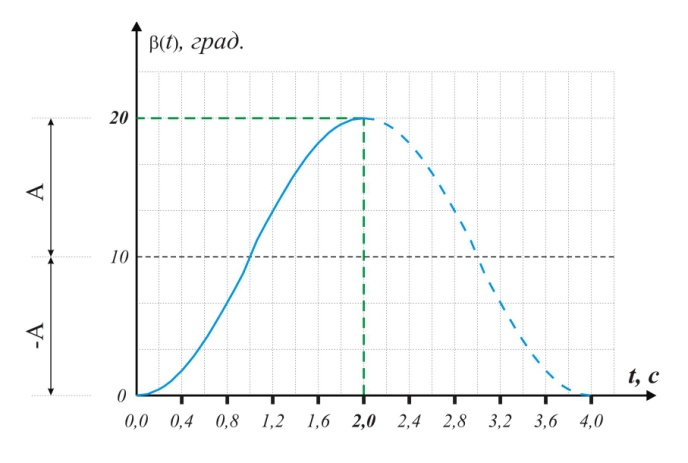
\includegraphics[keepaspectratio]{./src/pictures/retarget_equivalent_input_signals/20grad_2sec}
    \caption{Перенацеливание камеры на $q = 20^{\circ}$ за $t_\textit{п} = 2$ c}
    \label{retarget_20grad_2sec}
\end{figure}

Зная $t_{\textit{п} } = 2$ c, можем определить нужные нам параметры перенацеливания
с помощью (\ref{equiv_signal_frequency}),
(\ref{max_speed_for_equiv_signal}),
(\ref{max_acceleration_for_equiv_signal}):

$$
    \omega_{\beta.p} = \frac{\pi}{2} = 1.57 ~\textit{рад} \cdot \textit{с}^{-1}
$$
$$
    \dot{\beta}_{max} = 0.1745 \cdot 1.57 = 0.274 ~\textit{рад} \cdot \textit{c}^{-1}
$$
$$
    \ddot{\beta}_{max} = 15.7 \cdot 1.57 = 0.43 ~\textit{рад}  \cdot \textit{c}^{-2}
$$

\subsubsection{Перенацеливание, режим 2}

\textbf{Параметры:} $q = \frac{\pi}{4} ~\textit{рад}$ за $t_{\textit{п}} = 3 ~\textit{c}$

Представим данный участок (от $\beta_{H}$ до $\beta_{K}$) в виде синусоиды от
точки $-A_\textit{экв}$ до точки $+A_\textit{экв}$ на участке полупериода
(рис. \ref{retarget_45grad_3sec}), $A_\textit{экв}$ в данном случае равна
$\frac{q}{2} = \frac{\pi}{8} ~\textit{рад}$.

\begin{figure}[h!]
    \centering
    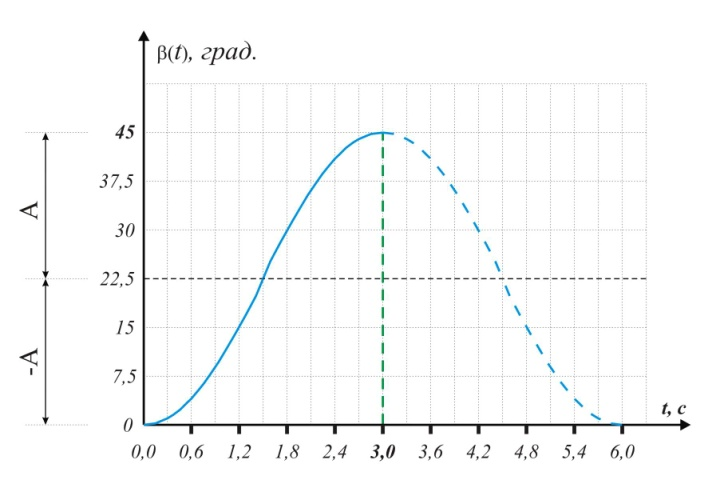
\includegraphics[keepaspectratio]{./src/pictures/retarget_equivalent_input_signals/45grad_3sec}
    \caption{Перенацеливание камеры на $q = 45^{\circ}$ за $t_\textit{п} = 3$ c}
    \label{retarget_45grad_3sec}
\end{figure}

Зная $t_{\textit{п} } = 3 ~\textit{c}$, можем определить нужные нам параметры перенацеливания
с помощью (\ref{equiv_signal_frequency}),
(\ref{max_speed_for_equiv_signal}),
(\ref{max_acceleration_for_equiv_signal}):

$$
    \omega_{\beta.p} = \frac{\pi}{3} = 1.047 ~\textit{рад} \cdot \textit{с}^{-1}
$$
$$
    \dot{\beta}_{max} = \frac{\pi}{8} \cdot \frac{\pi}{3} = 0.41 ~\textit{рад} \cdot \textit{с}^{-1}
$$
$$
    \ddot{\beta}_{max} = \frac{\pi}{8} \cdot \frac{\pi}{3} \cdot \frac{\pi}{3} = 0.431 ~\textit{рад} \cdot \textit{с}^{-2}
$$

\subsubsection{Перенацеливание, режим 3}

\textbf{Параметры:} $q = \frac{\pi}{2} ~\textit{рад}$ за $t_\textit{п} = 4.3 ~\textit{c}$

Представим данный участок (от $\beta_{H}$ до $\beta_{K}$) в виде синусоиды от точки
$-A_\textit{экв}$ до точки $+A_\textit{экв}$ на участке полупериода
(рис. \ref{retarget_90grad_4,3sec}), $A_\textit{экв}$ в данном случае
равна $\frac{q}{2} = \frac{\pi}{4} ~\textit{рад}$.

\begin{figure}[ht!]
    \centering
    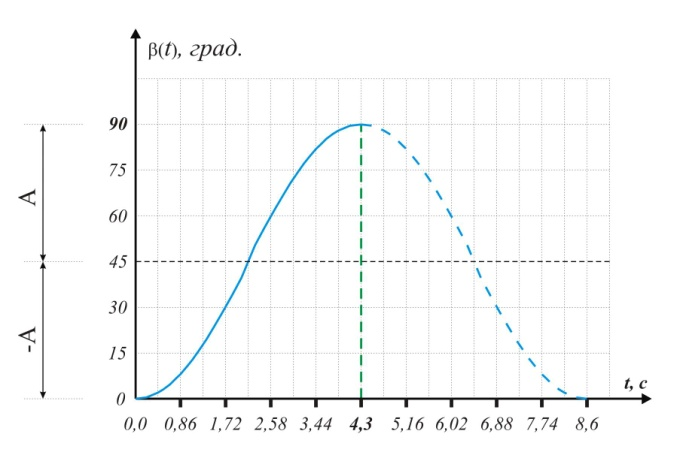
\includegraphics[keepaspectratio]{./src/pictures/retarget_equivalent_input_signals/90grad_4,3sec}
    \caption{Перенацеливание камеры на $q = 90^{\circ}$ за $t_\textit{п} = 4.3$ c}
    \label{retarget_90grad_4,3sec}
\end{figure}

Зная $t_{\textit{п} } = 4.3$ c, можем определить нужные нам параметры перенацеливания
с помощью (\ref{equiv_signal_frequency}),
(\ref{max_speed_for_equiv_signal}),
(\ref{max_acceleration_for_equiv_signal}):

$$
    \omega_{\beta.p} = \frac{\pi}{4.3} = 0.73 ~\textit{рад} \cdot \textit{с}^{-1}
$$
$$
    \dot{\beta}_{max} = \frac{\pi}{4} \cdot \frac{\pi}{4.3} = 0.574 ~\textit{рад} \cdot \textit{с}^{-1}
$$
$$
    \ddot{\beta}_{max} = \frac{\pi}{4} \cdot \frac{\pi}{4.3} \cdot \frac{\pi}{4.3} = 0.419 ~\textit{рад} \cdot \textit{с}^{-2}
$$

Таким образом,

Максимальная угловая скорость камеры:
\begin{equation}
    \dot{\beta}_{max} = 0.574 ~\textit{рад} \cdot \textit{с}^{-1}
\end{equation}

Максимальное ускорение камеры:
\begin{equation}
    \ddot{\beta}_{max} = 0.431 ~\textit{рад} \cdot \textit{с}^{-2}
\end{equation}

Расчет соответствующих параметров приводов для обеспечения параметров перенацеливания камеры:

Коэффициент $ K_{\beta} $  принято называть коэффициентом распределения заданной величины перемещения камеры на
звенья поворотного механизма (далее по тексту – коэффициент распределения).
Типовой коэффициент распределения при вышеприведенных инерционных и геометрических параметрах
системы, которые будем использовать при расчете требуемых ускорений нагрузок приводов:

\begin{equation}
    K_{\beta} = 2
\end{equation}

Максимальный коэффициент распределения, который будем использовать при расчете требуемых скоростей
нагрузок приводов, выберем с запасом:

\begin{equation}
    K_{\beta} = 3
\end{equation}

Максимальные требуемые скорости нагрузок приводов:
\begin{equation}
    \dot{\beta}_{max} = 0.574 \cdot 3 = 1.722 ~\textit{рад} \cdot \textit{с}^{-1}
\end{equation}

Максимальное требуемое ускорение нагрузок приводов:
\begin{equation}
    \ddot{\beta}_{max} = 0.431 \cdot 3 = 1.293 ~\textit{рад} \cdot \textit{с}^{-2}
\end{equation}

Максимальная требуемая величина углового перенацеливания нагрузки привода (с учетом максимальных
коэффициентов распределения):

\begin{equation}
    q_{max} = 3 \cdot \frac{\pi}{4} = \frac{3 \pi}{4}
\end{equation}

Таким образом, при проектировании приводных блоков необходимо обеспечить максимальные динамические
характеристики нагрузок на их выходных валах, представленные в (\ref{drive_parameters_tbl}).

\newpage
\subsubsection{Сводная таблица результатов}

\begin{table}[h!]
    \centering
    \begin{tabular}{|l|c|l|}
        \hline
        Параметр                                    & Обозначение      & Значение                                       \\
        \hline
        Напряжение питания                          & $U_1$            & $24 \textit{ В} $                              \\
        Шаг единичного углового перемещения нагрузки& $q_d$            & $ \le 1' $                                     \\
        Ресурс                                      &                  & $30000 \textit{ ч} $                           \\
        Диапазон углового перенацеливания нагрузки  & $q_{max}$        & $[-135^\circ .. 135^\circ] $                   \\
        Максимальная угловая скорость нагрузки      & $\dot{q}_{max}$  & $1.722 \textit{ рад} \cdot \textit{ c}^{-1}$   \\
        Максимальное ускорение нагрузки             & $\ddot{q}_{max}$ & $1.293 \textit{ рад} \cdot \textit{ c}^{-2}$   \\
        Момент инерции нагрузки                     & $J_{oy}$         & $3 ~\textit{ кг} \cdot \textit{ м}^2 $         \\
        \hline
    \end{tabular}
    \caption{Требуемые параметры привода}
    \label{drive_parameters_tbl}
\end{table}
